%%%%%%%%%%%%%%%%%%%%%%%%%%%%%%%%%%%%%%%%%%%%%%%%%%%%%%%%%%%%%%%%%%%%%%%%%%%%%%%
%
% Filename: paper.tex
% Author:   David Oniani
% Modified: May 05, 2020
%  _         _____   __  __
% | |    __ |_   _|__\ \/ /
% | |   / _` || |/ _ \\  /
% | |__| (_| || |  __//  \
% |_____\__,_||_|\___/_/\_\
%
%%%%%%%%%%%%%%%%%%%%%%%%%%%%%%%%%%%%%%%%%%%%%%%%%%%%%%%%%%%%%%%%%%%%%%%%%%%%%%%

%%%%%%%%%%%%%%%%%%%%%%%%%%%%%%%%%%%%%%%%%%%%%%%%%%%%%%%%%%%%%%%%%%%%%%%%%%%%%%%
% Document Definition
%%%%%%%%%%%%%%%%%%%%%%%%%%%%%%%%%%%%%%%%%%%%%%%%%%%%%%%%%%%%%%%%%%%%%%%%%%%%%%%

\documentclass[11pt]{article}

%%%%%%%%%%%%%%%%%%%%%%%%%%%%%%%%%%%%%%%%%%%%%%%%%%%%%%%%%%%%%%%%%%%%%%%%%%%%%%%
% Packages and Related Settings
%%%%%%%%%%%%%%%%%%%%%%%%%%%%%%%%%%%%%%%%%%%%%%%%%%%%%%%%%%%%%%%%%%%%%%%%%%%%%%%

% Global, document-wide settings
\usepackage[margin=1in]{geometry}
\usepackage[utf8]{inputenc}
\usepackage[english]{babel}

% Bibliography and references
\usepackage[backend=biber,sorting=none]{biblatex}
\addbibresource{references.bib}

% Other packages
\usepackage{booktabs}
\usepackage{fancyhdr}
\usepackage{hyperref}
\usepackage{mathtools}
\usepackage[cache=false]{minted}
\usepackage{tocloft}
\usepackage{tikz}

%%%%%%%%%%%%%%%%%%%%%%%%%%%%%%%%%%%%%%%%%%%%%%%%%%%%%%%%%%%%%%%%%%%%%%%%%%%%%%%
% Command Definitions and Redefinitions
%%%%%%%%%%%%%%%%%%%%%%%%%%%%%%%%%%%%%%%%%%%%%%%%%%%%%%%%%%%%%%%%%%%%%%%%%%%%%%%

% Magnitude
\DeclarePairedDelimiter\abs{\lvert}{\rvert}

% Line spacing is 1.5
\renewcommand{\baselinestretch}{1.5}

%%%%%%%%%%%%%%%%%%%%%%%%%%%%%%%%%%%%%%%%%%%%%%%%%%%%%%%%%%%%%%%%%%%%%%%%%%%%%%%
% Miscellaneous
%%%%%%%%%%%%%%%%%%%%%%%%%%%%%%%%%%%%%%%%%%%%%%%%%%%%%%%%%%%%%%%%%%%%%%%%%%%%%%%

% Setting stuff
\setlength{\parindent}{0pt}  % Remove indentations from paragraphs
\pagestyle{fancy}            % This allows to do fancy headers and footers
\fancyhf{}                   % No additional page numbering (or other stuff)
\cfoot{\thepage}             % Display page number at the bottom, in the center
\usemintedstyle{tango}       % Colorscheme for minted

% PDF information and nice-looking urls
\hypersetup{%
  pdfauthor={David Oniani},
  pdftitle={Cosine Similarity and Its Applications in the Domans of Artificial
    Intelligence},
  pdfsubject={Cosine Similarity, Artificial Intelligence, Natural Language
    Processing},
  pdfkeywords={Cosine Similarity, Artificial Intelligence, Natural Language
    Processing},
  pdflang={English},
  colorlinks=true,
  linkcolor={black!50!blue},
  citecolor={black!50!blue},
  urlcolor={black!50!blue}
}

% Put a header
\chead{\footnotesize{Cosine Similarity and Its Applications in the Domains of
  Artificial Intelligence}}
\lhead{\footnotesize{David Oniani}}

%%%%%%%%%%%%%%%%%%%%%%%%%%%%%%%%%%%%%%%%%%%%%%%%%%%%%%%%%%%%%%%%%%%%%%%%%%%%%%%
% Author(s), Title, and Date
%%%%%%%%%%%%%%%%%%%%%%%%%%%%%%%%%%%%%%%%%%%%%%%%%%%%%%%%%%%%%%%%%%%%%%%%%%%%%%%

% Author(s)
\author{David Oniani\\
        Luther College\\
        \href{mailto:oniada01@luther.edu}{oniada01@luther.edu}}

% Title
\title{\textbf{Cosine Similarity and Its Applications in the Domains of
  Artificial Intelligence}\\\color{black!50!blue}$<$ D R A F T $>$}

% Date
\date{\today}

%%%%%%%%%%%%%%%%%%%%%%%%%%%%%%%%%%%%%%%%%%%%%%%%%%%%%%%%%%%%%%%%%%%%%%%%%%%%%%%
% Beginning of the Document
%%%%%%%%%%%%%%%%%%%%%%%%%%%%%%%%%%%%%%%%%%%%%%%%%%%%%%%%%%%%%%%%%%%%%%%%%%%%%%%

\begin{document}
\maketitle

%%%%%%%%%%%%%%%%%%%%%%%%%%%%%%%%%%%%%%%%%%%%%%%%%%%%%%%%%%%%%%%%%%%%%%%%%%%%%%%
% Abstract
%%%%%%%%%%%%%%%%%%%%%%%%%%%%%%%%%%%%%%%%%%%%%%%%%%%%%%%%%%%%%%%%%%%%%%%%%%%%%%%

\begin{abstract}
  \noindent Choosing the right metric~\cite{thomas2020} can be crucial to
  designing performant artificial intelligence models. Thousands of packages
  and libraries have been built and written just for providing these metrics.
  Cosine similarity is one of many metrics used extensively in natural language
  processing (NLP) tasks. The paper will introduce the technique and discuss
  its advantages and disadvantages as well as compare it to other approaches.
  Additionally, sample implementations of the technique will also be provided.
\end{abstract}

%%%%%%%%%%%%%%%%%%%%%%%%%%%%%%%%%%%%%%%%%%%%%%%%%%%%%%%%%%%%%%%%%%%%%%%%%%%%%%%
% Introduction
%%%%%%%%%%%%%%%%%%%%%%%%%%%%%%%%%%%%%%%%%%%%%%%%%%%%%%%%%%%%%%%%%%%%%%%%%%%%%%%

\section{Introduction}

There are many approaches for determining whether two texts are semantically
similar to each other. Cosine similarity is one of those methods. Derived from
the law of cosines~\cite{wikicosineproof}, the technique is now widely used in
natural language processing (and other) problems.

\bigskip

In order to understand how cosine similarity works, let us first discuss how a
text document can be modeled.

\subsection{Text Document Modeling}

There several ways in which a text document can be modeled. This includes a
\textit{bag-of-words} modeling, where the frequency of a term in a text
document represents its weight and \textit{tf-idf} vectorization. The primary
goal of text document modeling is to transform the textual data into the
numeric data (in this case, term vectors). Once the numeric data is obtained,
we can then apply mathematical techniques including text semantic similarity
approaches such as cosine similarity in order to compare if two documents are
similar to each other.

\subsection{Cosine Similarity}

Cosine similarity is a measure of similarity between two non-zero vectors of an
inner product space that measures the cosine of the angle between
them~\cite{wikicosine}. For two vectors \(\vec{a}\) and \(\vec{b}\),
the cosine can be computed as
\(\vec{a} \cdot \vec{b} = \abs{\vec{a}}\abs{\vec{b}}\cos\theta\),
where \(\theta\) is the angle between the vectors. This is also known as the
Euclidean dot product formula.
The cosine of two vectors can also be computed using their coordinates:
if \(\vec{a} = \begin{bmatrix}a_1 \\ a_2\end{bmatrix}\) and
\(\vec{b} = \begin{bmatrix}b_1 \\ b_2\end{bmatrix}\), then
\(\vec{a} \cdot \vec{b} = a_1b_1 + a_2b_2\). Hence, for two vectors \(\vec{a}\)
and \(\vec{b}\) with coordinates \(a_1, a_2\) and \(b_1, b_2\) respectively,
the following holds:

\[\vec{a} \cdot \vec{b} = \abs{\vec{a}}\abs{\vec{b}}\cos\theta = a_1b_1 + a_2b_2\]

\bigskip

If the vector coordinates are known, then one can also compute the magnitude of
the vector. For vector
\(\vec{x} = \begin{bmatrix}x_1 \\ x_2 \\ \dots \\ x_n\end{bmatrix}\),
the magnitude is \(\sqrt{x_1^2 + x_2^2 + \cdots + x_n^2}\). Hence, if we have two
vectors \(\vec{a} = \begin{bmatrix}a_1 \\ a_2 \\ \dots \\ a_n\end{bmatrix}\) and
\(\vec{b} = \begin{bmatrix}b_1 \\ b_2 \\ \dots \\ b_n\end{bmatrix}\), then the
cosine of an angle between them is:

\[ \cos\theta = \dfrac{a_1b_1 + a_2b_2 + \cdots + a_nb_n}{\sqrt{a_1^2 + a_2^2 + \cdots + a_n^2}\sqrt{b_1^2 + b_2^2 + \cdots + b_n^2}} \]

In other words, if we have two vectors with all coordinates specified, it is
possible to compute the cosine similarity between them.

\subsection{Example}

As an example, consider two vectors
\(\vec{a} = \begin{bmatrix}3 \\ 4\end{bmatrix}\)
and \(\vec{b} = \begin{bmatrix}5 \\ 12\end{bmatrix}\).
Then the magnitude of \(a\) is \(\sqrt{3^2 + 4^2} = 5\) and the magnitude of
\(b\) is \(\sqrt{5^2 + 12^2} = 13\). It follows that
\(\vec{a} \cdot \vec{b} = 15 + 48 = 63\) and
\(\abs{\vec{a}} \times \abs{\vec{b}} = 5 \times 13 = 65\). Therefore, the
cosine of an angle between the vectors is \(\dfrac{63}{65} \approx 0.969\)
which is the similarity measure between these two vectors.

\bigskip

For those who like to think visually, below is the plot from which one could
derive the cosine of the angle $\theta$ (e.g., by applying the law of cosines).

\begin{figure}[H]
  \begin{center}
    % TikZ picture with origin upper left
    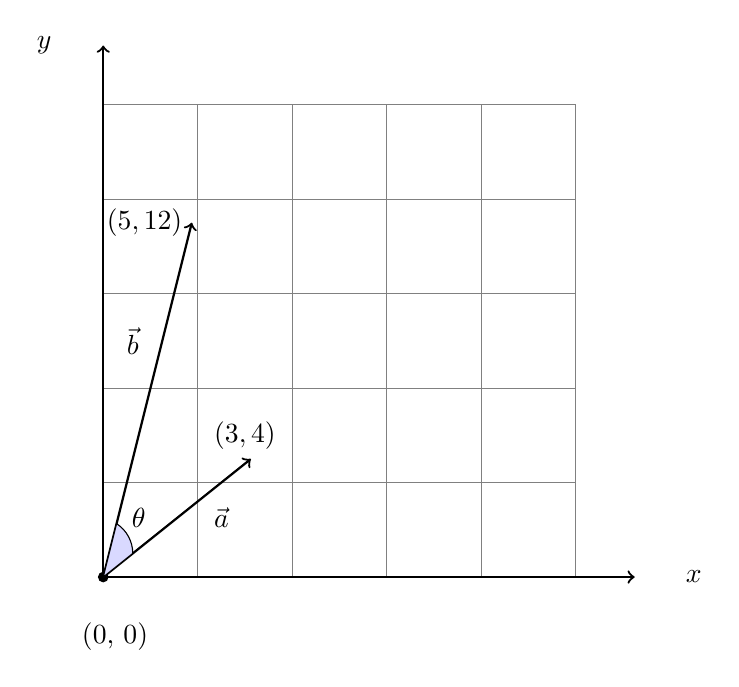
\begin{tikzpicture}[yscale=-1, scale=1.5]
      % 4x4 grid
      \draw[step=0.8cm,gray,very thin] (0,0) grid (4,4);

      % Origin
      \draw [fill=black] (0,4) circle (0.04);
      \node at (0.1,4.5) {(0, 0)};

      % x-axis
      \draw [thick,->] (0,4) -- (0,-0.5);
      \node at (-0.5,-0.5) {$y$};

      % y-axis
      \draw [thick,->] (0,4) -- (4.5,4);
      \node at (5,4) {$x$};

      % Points
      \node at (0.35,1) {$(5, 12)$};
      \node at (1.2,2.8) {$(3, 4)$};

      % Vectors
      \draw [thick,->] (0,4) -- (1.25,3);
      \node at (1,3.5) {$\vec{a}$};

      \draw [thick,->] (0,4) -- (0.75,1);
      \node at (0.25,2) {$\vec{b}$};

      % Angle
      \filldraw[fill=blue!15] (0,4) -- (2.5mm,3.8) arc (0:-57:3mm) -- cycle;
      \node at (0.3,3.5) {$\theta$};
    \end{tikzpicture}
  \end{center}
  \caption{Vector Cosine Illustration.}
\end{figure}


%%%%%%%%%%%%%%%%%%%%%%%%%%%%%%%%%%%%%%%%%%%%%%%%%%%%%%%%%%%%%%%%%%%%%%%%%%%%%%%
% Applications
%%%%%%%%%%%%%%%%%%%%%%%%%%%%%%%%%%%%%%%%%%%%%%%%%%%%%%%%%%%%%%%%%%%%%%%%%%%%%%%

\section{Applications}

Cosine similarity is one of the most commonly used approaches in calculating
semantic similarity of texts. Therefore, it is naturally employed in natural
language processing tasks. Many NLP applications need to compute the semantic
similarity between two short texts. Search engines, for instance, need to model
the relevance of a document to a query on the semantic level. Similarly, Q\&A
websites such as Stack Overflow and Quora need to determine whether a question
has already been asked before. Cosine similarity is usually one of the typical
first solutions to such problems.

\bigskip

Suppose that we have two documents \(D_1\) and \(D_2\) modeled as term vectors
\(\vec{t_1}\) and \(\vec{t_2}\) respectively. Then the similarity of two
documents corresponds to the correlation between the vectors and can be
quantified as a cosine of the angle between the vectors. Thus, the similarity
formula~\cite{huang2008} is:

\[SIM_C(\vec{t_1}, \vec{t_2}) = \dfrac{\vec{t_1} \cdot
  \vec{t_2}}{\abs{\vec{t_1}} \times \abs{\vec{t_2}}}.\]

As a result, the similarity value is non-negative, bounded by the closed
interval \([0,1]\).

\bigskip

It is important to note that the metric is a measurement of orientation and not
the magnitude. It can be thought of as a comparison of documents on a
normalized space since it does not only consider the magnitude of word counts
of each document, but also the angle between the documents.

\bigskip

Below find a simple Python implementation of cosine similarity.

\begin{figure}[H]
  \begin{minted}[fontsize=\small,frame=single]{python}
  import numpy as np

  def cosine_similarity(a: np.array, b: np.array) -> float:
      """Returns the cosine similarity value of two vectors."""

      dot_product: float = np.dot(a, b)
      magnitude_a: float = np.linalg.norm(a)
      magnitude_b: float = np.linalg.norm(b)
      similarity: float = dot_product / (magnitude_a * magnitude_b)

      return similarity


  if __name__ == "__main__":
      a: np.array = np.array([1, 0, 1, 0, 1, 1, 1, 1, 1, 1, 1])
      b: np.array = np.array([0, 2, 1, 0, 1, 3, 0, 0, 0, 1, 0])
      print(cosine_similarity(a, b))  # Prints out 0.5
  \end{minted}
  \caption{Sample Python Implementation of Cosine Similarity.}
\end{figure}

The program is fairly simplistic (yet performant) and as shown above,
\mintinline{python}{cosine_similarity} function takes two vectors and prints
out the cosine similarity between them. Vectors \mintinline{python}{a} and
\mintinline{python}{b} can be thought of as vectorized text (i.e., the
vectorization algorithm has already been applied to two texts).

%%%%%%%%%%%%%%%%%%%%%%%%%%%%%%%%%%%%%%%%%%%%%%%%%%%%%%%%%%%%%%%%%%%%%%%%%%%%%%%
% Comparison to Other Approaches
%%%%%%%%%%%%%%%%%%%%%%%%%%%%%%%%%%%%%%%%%%%%%%%%%%%%%%%%%%%%%%%%%%%%%%%%%%%%%%%

\section{Performance and Comparison to Other Approaches}

Performance of cosine similarity can be altered by the approach used for
vectorization~\cite{sitikhu2019} (e.g., tf-idf vectorization might yield better
results than Word2Vec vectorization). Needless to say that the right
vectorization strategy could drastically increase the performance, while the
poor vectorization will, unsurprisingly, result in the poor performance.

\medskip

There are many other approaches for finding semantic similarity between the
texts. The recent advancements in the domains of artificial intelligence and
natural language processing allowed for development of models such as
BERT~\cite{turc2019}, BioBERT~\cite{btz682}, and Universal Sentence Encoder
(USE)~\cite{use}, all of which can be used for high-accuracy text semantic
similarity score computations. The advantage of the cosine similarity, however,
is its simplicity and the fact that one could run it over massive datasets.
Doing the same with models like BioBERT could possibly take a lot of time and
hence, be highly inefficient.

%%%%%%%%%%%%%%%%%%%%%%%%%%%%%%%%%%%%%%%%%%%%%%%%%%%%%%%%%%%%%%%%%%%%%%%%%%%%%%%
% Current Work
%%%%%%%%%%%%%%%%%%%%%%%%%%%%%%%%%%%%%%%%%%%%%%%%%%%%%%%%%%%%%%%%%%%%%%%%%%%%%%%

\section{Current Work}

Cosine similarity is very much used in the modern, state-of-the-art papers,
such as ones cited in this paper. Its flexibility allows one to apply it under
virtually any settings, as long as documents can be represented as vectors.
Besides, it is widely used for benchmarking purposes and is usually a standard
against which the new approaches are tested.

%%%%%%%%%%%%%%%%%%%%%%%%%%%%%%%%%%%%%%%%%%%%%%%%%%%%%%%%%%%%%%%%%%%%%%%%%%%%%%%
% Summary
%%%%%%%%%%%%%%%%%%%%%%%%%%%%%%%%%%%%%%%%%%%%%%%%%%%%%%%%%%%%%%%%%%%%%%%%%%%%%%%

\section{Summary}

We have introduced cosine similarity and walked through examples to strengthen
the understanding of the concept. Besides, we discussed the importance of
cosine similarity in the domains of artificial intelligence and natural
language processing and its prevalence in the state-of-the-art work. Sample
Python implementation of the algorithm was also provided.

%%%%%%%%%%%%%%%%%%%%%%%%%%%%%%%%%%%%%%%%%%%%%%%%%%%%%%%%%%%%%%%%%%%%%%%%%%%%%%%
% Bibliography and References
%%%%%%%%%%%%%%%%%%%%%%%%%%%%%%%%%%%%%%%%%%%%%%%%%%%%%%%%%%%%%%%%%%%%%%%%%%%%%%%

\printbibliography[heading=bibintoc]

%%%%%%%%%%%%%%%%%%%%%%%%%%%%%%%%%%%%%%%%%%%%%%%%%%%%%%%%%%%%%%%%%%%%%%%%%%%%%%%
% The End of the Document
%%%%%%%%%%%%%%%%%%%%%%%%%%%%%%%%%%%%%%%%%%%%%%%%%%%%%%%%%%%%%%%%%%%%%%%%%%%%%%%

\end{document}
